\documentclass[a4paper,12pt]{article}
\usepackage{graphicx}
\usepackage{geometry}
\usepackage{fancyhdr}
\usepackage{float}
\usepackage{amsmath}
% \usepackage{hyperref}
\usepackage{geometry}
\usepackage{natbib}
\usepackage{project}
\usepackage{tikz}
\usepackage{wrapfig}
\usepackage{subcaption}
\usetikzlibrary{positioning, shapes.geometric, arrows}

\usepackage[colorlinks=true, linkcolor=blue, citecolor=blue, urlcolor=blue]{hyperref}
% \geometry{a4paper, margin=1in}
\geometry{margin=1in}
% Configure the header using fancyhdr
\pagestyle{fancy}
\fancyhf{} % Clear all header and footer fields
\fancyhead[L]{06.01.2025} % Left-aligned header
% \fancyhead[C]{MADE Data Report --- Asheer Ali (22993810)} % Center-aligned header
\fancyhead[R]{\thepage} % Right-aligned header (page number)
\renewcommand{\headrulewidth}{0.4pt} % Line under header

% Title configuration
\title{Traffic Crash Patterns: Assessing the Influence of Various Factors}
\author{} % Remove author to suppress it
\date{} % Empty date to suppress it

\begin{document}

% Custom title block
\begin{center}
    \textbf{\Large Traffic Crash Patterns: Assessing the Influence of Human Factors} \\[1em]
    Asheer Ali (22993810) \hspace{2cm} 16.01.2025
\end{center}

	\section{Introduction}
    Traffic crashes are a big concern that needs attention and required a comprehensive analysis in order to identify the critical issues. This report investigates to main questions. 
		\begin{itemize}
			\item How do driver characteristics correlate with injury severity in crashes?
			\item What types of vehicles are most involved in crashes?	\end{itemize}
	
    Knowing these patterns may make roads safer and reduce serious accidents.

\section{Data Sources}
\subsection{Descriptions of Data Sources}
\begin{itemize}
    \item \textbf{Traffic Crashes - People:} This dataset contains details of individuals involved in traffic incidents, including demographics, safety equipment use, and injury severity \cite{traffic_crashes_people}.
    
    \begin{figure}[H]
        \centering
        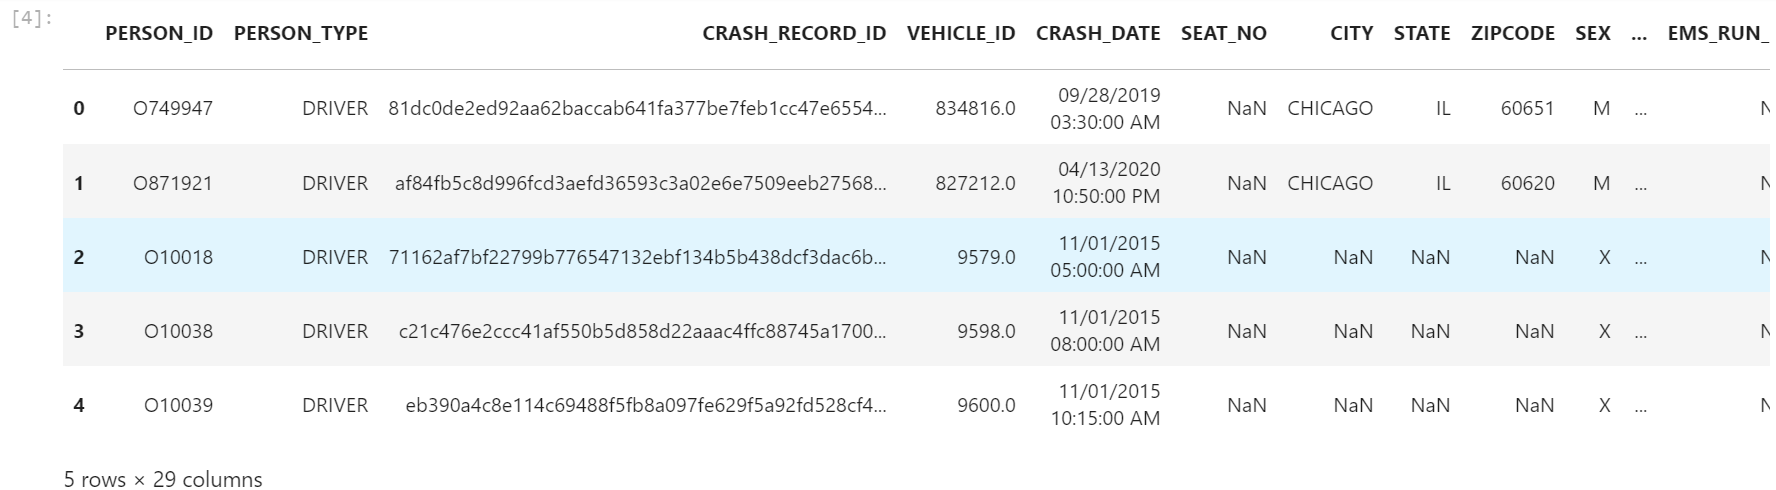
\includegraphics[width=1\linewidth]{images/dataset1.png}
        \caption{First 5 rows of traffic crashes people dataset}
        \label{fig:people}
    \end{figure}
    
    \item \textbf{Traffic Crashes - Vehicles:} Provides records of vehicles involved in crashes, including type, direction, and damage details \cite{traffic_crashes_vehicles}.
    
    \begin{figure}[H]
        \centering
        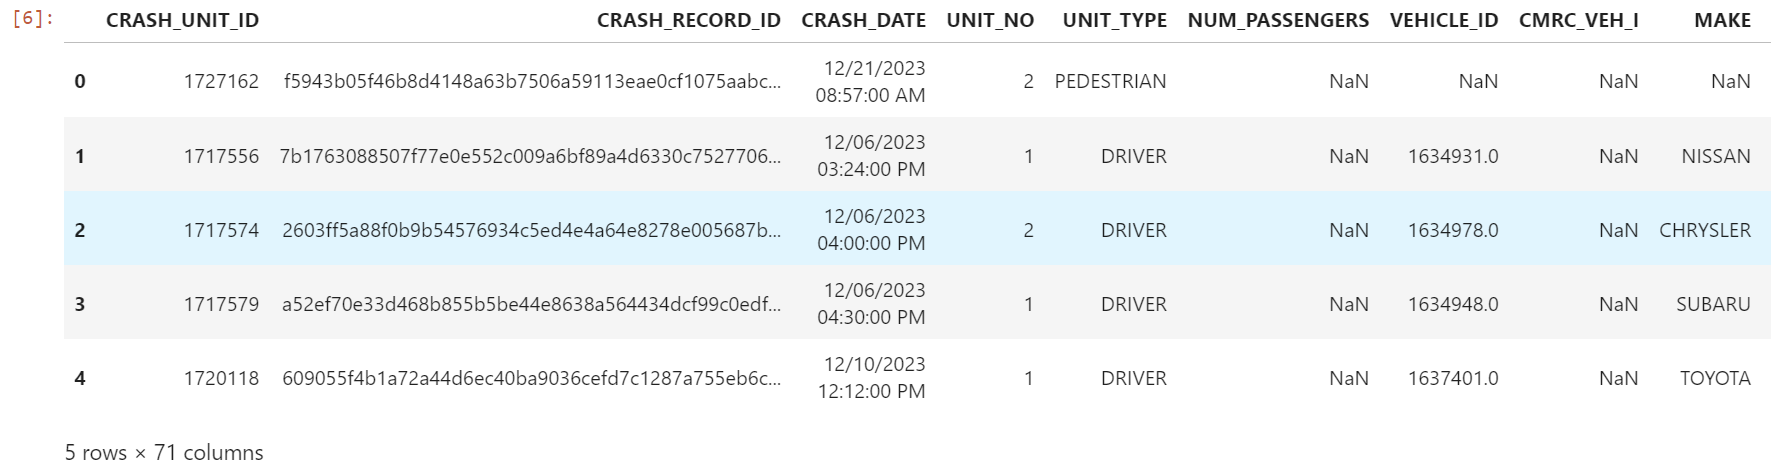
\includegraphics[width=1\linewidth]{images/dataset2.png}
        \caption{First 5 rows of traffic crashes vehicle dataset}
        \label{fig:vehicles}
    \end{figure}
\end{itemize}

\subsection{Structure and Quality of Data Sources}
\begin{itemize}
    \item \textbf{People Dataset:} Contains individual-level data with fields for demographics, safety equipment use, and injury severity. Missing values exist but can be handled through removing the rows with Nan values, as the nan values are not present that much in the selected columns. \cite{github_repo}.
    \item \textbf{Vehicle Dataset:} Vehicle-level data with fields for type, damage, and direction. Data quality is high, with minimal missing values.
\end{itemize}

\subsection{Licenses and Permissions}
Both datasets are publicly available under open-data licenses, allowing use with proper attribution \cite{traffic_crashes_people, traffic_crashes_vehicles}.

\section{Data Pipeline}
The data pipeline is implemented using Python and consists of the following steps:
\begin{itemize}
    \item \textbf{Extractor:} Downloads CSV files from the given URLs.
    \item \textbf{Transformer:} Processes the data with:
        \begin{itemize}
            \item Removing unnecessary columns.
            \item Handling missing values through imputation.
            \item Standardizing date formats for consistency.
        \end{itemize}
    \item \textbf{Loader:} Stores the cleaned datasets in an SQLite database for efficient access.
\end{itemize}

\begin{figure}
    \centering
    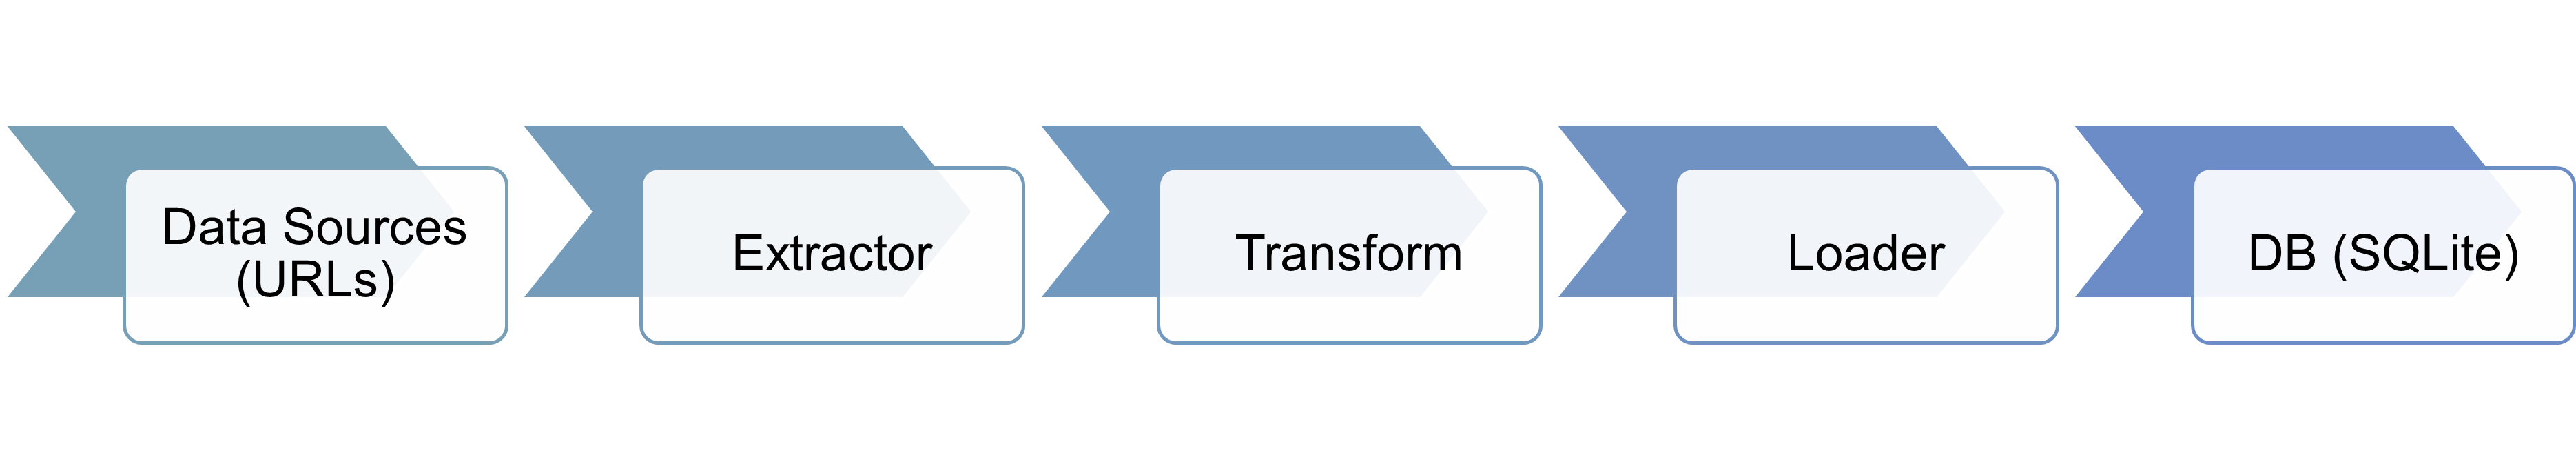
\includegraphics[width=1\linewidth]{images/Picture1.png}
    \caption{ETL Pipeline}
    \label{fig:ETL-pipeline}
\end{figure}

\section{Results and Limitations}
\subsection{Results}
\begin{itemize}
    \item Cleaned datasets stored in SQLite database.
    \item Data ready for analysis to address project questions about injury severity and crash patterns.
\end{itemize}

\subsection{Limitations}
\begin{itemize}
    \item Missing data for certain fields may impact analysis accuracy.

\end{itemize}


\newpage
\section{Questions}

\subsection{How do driver characteristics correlate with injury severity in crashes?}

\begin{figure}
    \centering
    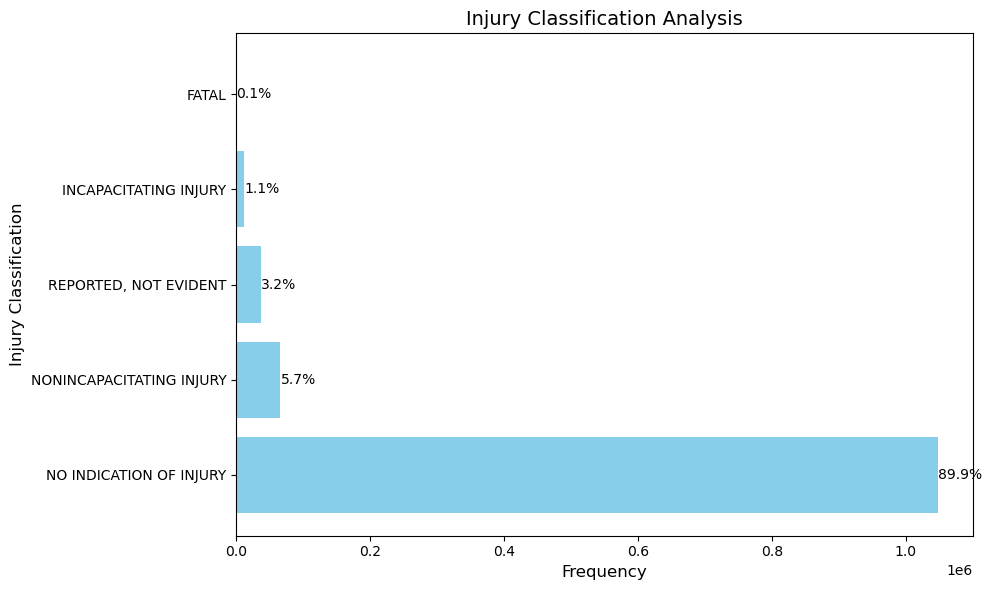
\includegraphics[width=0.75\linewidth]{images/injury-classification-analysis.png}
    \caption{Injury Classification Analysis}
    \label{fig:3.1}
\end{figure}

To find out how driver characteristics affect injury severity in crashes, we use the age, sex, and injury classification columns for our analysis and polt 3 graphs in as shown in figures \ref{fig:3.1}, \ref{fig:3.2}, and \ref{fig:3.3}.
\subsubsection{Key Findings}

\textbf{Injury Types:}
As Shown in \ref{fig:3.1} Most crashes did not show any signs of injury (89. 9\%). A small number of crashes had minor injuries (5. 7\%) or nonevident injuries (3. 2\%). Fatal crashes were very rare (0.1\%).

This means most crashes are not very severe, but even rare severe crashes need attention. 


\textbf{Age and Injury Severity:}
When I checked the link between age and injury severity, I found:

\begin{itemize}
    \item Severe injuries, like fatal or incapacitating ones, happened to drivers of all ages, but the average age was about 40 years.
    \item Younger drivers had more crashes with "No Indication of Injury," but age alone does not fully explain injury severity.
\end{itemize}

\textbf{Gender and Severe Crashes:}
For severe crashes (fatal and incapacitating):

\begin{itemize}
    \item Male drivers were in 61.7\% of these crashes.
    \item Female drivers were in 38.1\%.
    \item A small percentage (0.2\%) of crashes had other gender recorded.
\end{itemize}
Male drivers seem to have more severe crashes \ref{fig:3.3}, which could be due to behavior or exposure. 


Safety programs can focus on younger and male drivers to lower severe crashes. It is also important to study how other factors, like road conditions or vehicle types, might affect crashes.

\begin{figure}[ht!]
	\centering
	\begin{subfigure}[t]{0.48\textwidth}
		\centering
		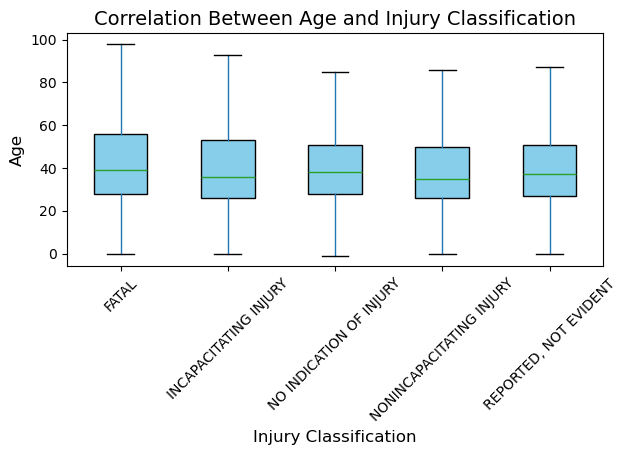
\includegraphics[width=\textwidth]{images/age-injury-classification.png} % Image file added
    \caption{Correlation between age and injury classification.}
    \label{fig:3.2}
	\end{subfigure}
	\hfill
	\begin{subfigure}[t]{0.48\textwidth}
		\centering
		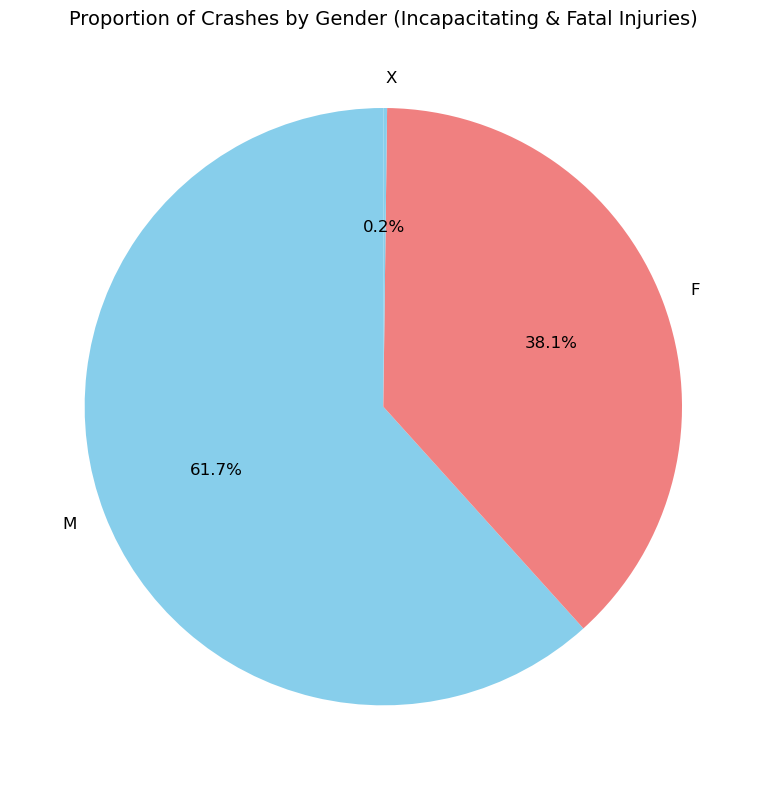
\includegraphics[width=\textwidth]{images/crashes-by-gender.png} % Image file added
    \caption{Proportion of crashes by gender (incapacitating and fatal injuries).}
    \label{fig:3.3}
    \end{subfigure}
	\caption{Comparison of Top Causes of Death and Their Trends}
\end{figure}





\begin{figure}
    \centering
    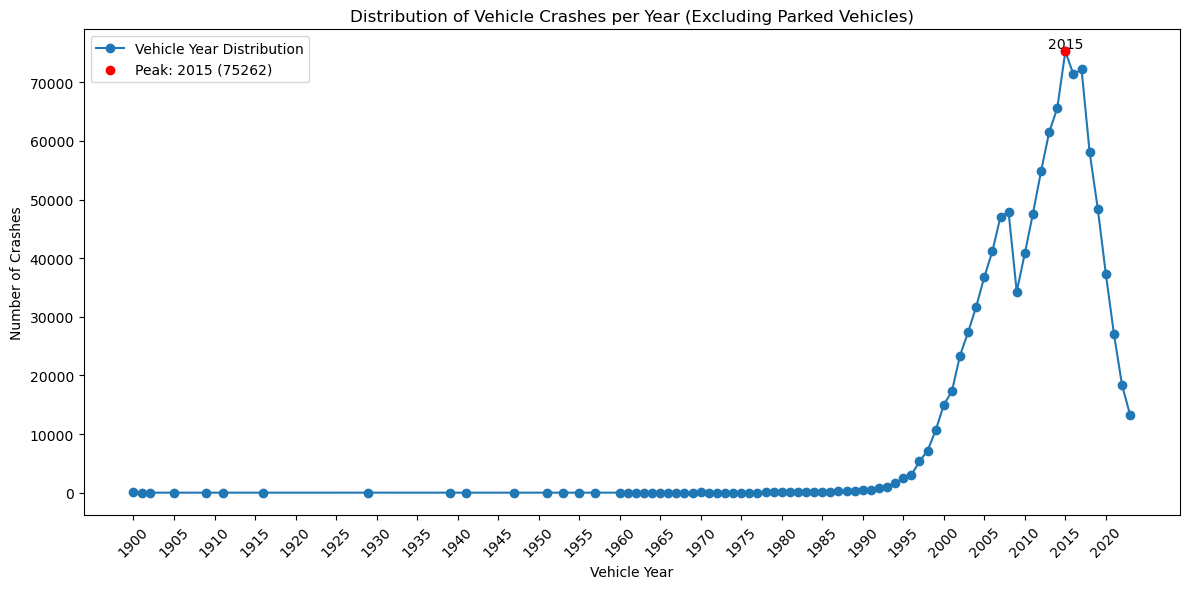
\includegraphics[width=0.75\linewidth]{images/vehicle-crashes-per-year.png}
    \caption{Distribution of Vehicle Crashes per Year (Excluding Parked Vehicles)}
    \label{fig:3.4}
\end{figure}
\subsection{What types of vehicles are most involved in crashes?}

\subsubsection{Findings:}
\textbf{Top 3 Vehicles with Most Crashes in 2015:}
\begin{itemize}
    \item \textbf{NISSAN ROGUE:} 2,329 crashes.
    \item \textbf{CHRYSLER 200:} 2,000 crashes.
    \item \textbf{JEEP CHEROKEE:} 1,884 crashes.
\end{itemize}
These vehicles had the most accidents in one year.

\subsubsection{Vehicle with Most Crashes Overall:}
\begin{itemize}
    \item \textbf{HONDA CIVIC:} 27,536 crashes in total.
\end{itemize}
This is the car with the highest number of crashes ever.



\begin{figure}
    \centering
    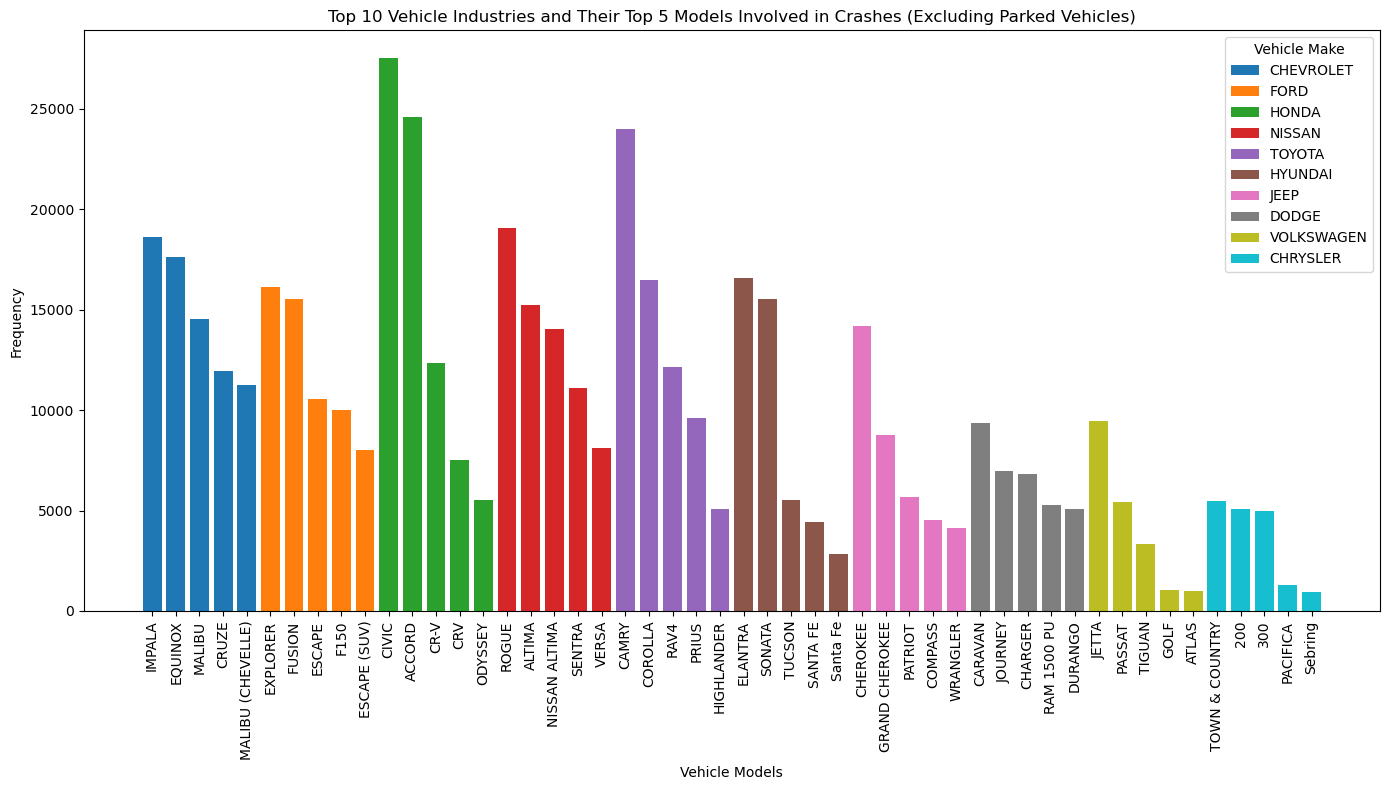
\includegraphics[width=0.75\linewidth]{images/vehicle-industries-in-crashes.png}
    \caption{Top 10 Vehicle Industries and Their Top 5 Models Involved in Crashes (Excluding Parked Vehicles)}
    \label{fig:3.5}
\end{figure}
\subsubsection{Observations:}
Cars from big brands like Nissan, Chrysler, and Honda are in more crashes. This may be because they are very popular. In 2015, some models had their highest crash numbers.



\section{Conclusion}

There are links between certain death rates and indicators of chronic diseases although the strength of these associations varies per condition. While cancer and mental health have weaker association with the death rates, conditions like diabetes and cardiovascular diseases have a large positive correlation with the death rates. Furthermore, the examination of the leading causes of deaths from 2020 to 2023 indicated that, although chronic conditions continued to rank among the primary causes of death, year-to-year variations may have been impacted by outside variables or other causes.

\vspace{1em}

Although the deeper dive into the datasets highlighted the associations among the death rates and disease prevalence, this research does not support the idea of causality. It can be difficult to conclude the precise role of the chronic diseases alone because of the potential influence of outside factors on the trends illustrated. Moreover, demographics, lifestyle, and healthcare quality may all have an independent role on the death rates.

\vspace{1em}

Following are the limitations:
\begin{itemize}
	\item The analysis assumes linear relationships, which may not fully capture more complex patterns or interactions between variables.
	\item The dataset only considers shared years between datasets, which may exclude relevant trends over longer periods.
	\item Outliers and noise in the data were not deeply analyzed, potentially affecting the robustness of the results.
	\item The focus was on the top causes of death, which might overlook important secondary contributors.
\end{itemize}



\section{Conclusion}

The data reveals key insights into traffic crash patterns and their relationships with driver characteristics, vehicle types, and crash severity. Most crashes do not involve injuries, with 89.9\% showing no indication of injury. However, attention must be given to severe crashes, even though they are rare. Drivers of all ages are involved in severe injuries, but the average age is around 40 years. Gender analysis highlights that male drivers are involved in a majority of severe crashes, indicating possible behavioral or exposure-related factors.

Popular vehicle models such as the Honda Civic, Nissan Rogue, and Chrysler 200 frequently appear in crash records. While the high crash numbers for these models may be linked to their popularity, further investigation into vehicle safety features and usage conditions is essential.

\vspace{12pt}
\textbf{Limitations}
\begin{itemize}
    \item The analysis assumes linear relationships, which might not capture complex interactions.
    \item Missing data and limited variables like road conditions and vehicle maintenance were not deeply explored.
    \item Results are based on available datasets and may not represent all contributing factors to crashes.
\end{itemize}

Overall, the findings suggest targeting safety programs for male drivers and younger drivers to mitigate severe crashes and exploring additional factors such as road and vehicle conditions for a comprehensive safety strategy.





\section{References}
\bibliographystyle{plain}
\bibliography{reference}
\end{document}
